\documentclass[11pt,a4paper]{article}

\usepackage{mathtext}

\usepackage[T1,T2A]{fontenc}

\usepackage[utf8]{inputenc}
\usepackage[english,ukrainian]{babel}

\usepackage{graphicx}
\graphicspath{ {./images/} }
\usepackage{float}
\usepackage{hyperref}

\author{Павло Токарєв, 4 курс, група МФ-41}
\title{Мережева симуляція}

\begin{document}
\maketitle

\tableofcontents

\section{Завдання}

Розробити модель мережі та декілька стратегій обробки черг маршрутування
і балансування навантаження між каналами зв'язку і 
методом порівняння визначити найбільш ефективну їх 
комбінацію з точки зору утилізації ресурсів мережі 
(пропускної здатності, величини черг повідомлень на вузлах)
і, за можливості, часу доставки пакетів та різних типів трафіку.

\section{Що зроблено}

Розроблений рушій для симуляції \footnote{event\_loop.py}, фреймворк  \footnote{framework.py} для симуляції мереж на основі \emph{EventLoop} класа, модель мережі та декілька комбінацій стратегій обробки черг і балансування.

\section{Рушій}

Рушій розроблено на основі системи подій (event-based simulation) 
та функцій-обробників цих подій. Цикл обробки подій наповнюється
початковими подіями, які сортуються за часом їх появи. Коли
подія повинна бути оброблена, визивається функція, що 
відповідає типу події.

Даний цикл продовжується до тих пір, поки не закінчаться події
у черзі або не буде перевищений час виконання симуляції 
(який можна не вказувати, якщо Ви знаєте, що ця система подій сходиться/закінчується).

Даний рушій розроблявся з розрахунком на обмеження 
роздільної здатності часу до наносекунди --- користувацька функція можете повернути не цілий час появи повідомлення, але це теоретично може вплинути на продуктивність симуляції через операції над числами з рухомою комою.

\section{Мережа}

Мережа визначається наборами вузлів та каналів між ними. Вузли у свою чергу визначаються своїм IP (на даний момент задля простоти вибрано ціле число), чергою повідомлень, набором інтерфейсів (вихідні канали до усіх сусідів) та таблицею маршрутизації. Канали пов'язують два вузла, мають чергу повідомлень, та швидкість (наносекунд/байт).

Таблиці маршрутизації статичні, та формуються до початку конкретно симуляції.
Стратегієя побудови цих таблиць наступна: кожен вузел мережі формує 
спеціальний пакет у вигляді події для кожного 
з'єднання, що він має. У цьому пакеті він повідомляє про себе: його IP та час до нього.
Коли цей пакет доходить до якогось вузла, цей вузол додає запис до таблиці маршрутизації про те, 
через який інтерфейс цей пакет був надісланий, тобто через який інтейфейс IP даного вузла може бути доступний, та розсилає 
таке ж повідомлення до усіх своїх сусідів. Якщо цей IP та інтерфейс 
вже є у таблиці, таблиця може бути модифікована тільки якщо у таблиці
метрика для інтерфейса більша за нову; повідомлення до сусідів не відправляється.
Повідомлення про вузол просто викидаються, якщо воно повертається до його джерела.

Так як вузли не розсилають повідомлення сусідам у разі запису у таблиці 
(тобто є захист від циклів), алгоритм формування таблиць сходиться.

\subsection{Система подій}
Симуляція мережі базується на наступних типах подій:
\begin{itemize}
\item зупинки часу: періодична подія, що дозволяє збирати статистику мережі.
\item нового з'єднання: створює набір нових пакетів на вузлі відправки;
\item нового пакета: додає пакет у чергу на маршрутизацію;
\item маршрутизації: оброблює один пакет з черги вузла, додає пакет у якийсь з каналів,
або поглинає, якщо цей пакет адресовано цьому вузлу;
\item передачі пакета: подія передачі пакета у якомусь каналі, може бути зіпсовано подією помилки;
\item помилки передачі у каналі: позначає канал таким, у якому відбулася помилка передачі у даний час;
прибирається наступним пакетом.
\end{itemize}

Усі ці події оброблюються методами класу \emph{Networking}, 
який користувач може замінити на свій підклас.

Виникнення усіх подій (якщо не зазначено іншого) симулюється окремим 
пуасонівським процесом зі своєю інтенсивністю.

Генерація появи нових повідомлень у мережі наразі не регулюється
рисами вузлів (як от вага вузла, наприклад, для симуляції реального навантаження, штибу популярних сервісів), окрім як рисами клієнта та сервера (за замовчуванням вузол є і клієнтом, і сервером, і роутером, що значить, що повідомлення генеруються між усіма вузлами).

\section{Алгоритми та стратегії}

\subsection{FIFO обробка черги}
Обирає найдавніший (перший у списку) елемент черги.

\subsection{LIFO обробка черг}
Обирає наймолодший (останній у списку) елемент черги.

\subsection{FIRST маршрутизація}
Перший канал із запису маршрутизації для даного IP.

\subsection{RANDOM маршрутизація}
Канал для передачі повідомлення вибирається випадково та рівнозважено з наявних у записі маршрутизації.

\subsection{WEIGHT RANDOM маршрутизація}
Те саме, що і у RANDOM, але
шанс вибору каналу для передачі повідомлення є більшим для тих каналів, для
яких більша метрика (кумулятивний час на байт).

\section{Результати}

Далі наведені результати симуляцій для наступної мережі:

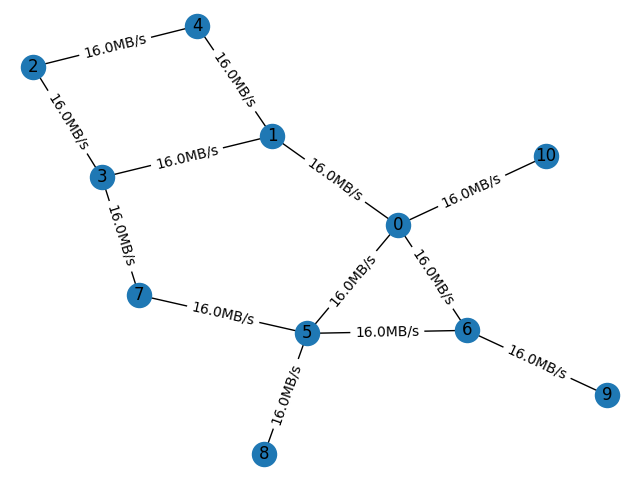
\includegraphics[width=\textwidth]{graph}

Усі симуляції відбувалися напротязі \emph{1 секунди}, з кроком збору статистики \emph{50 мілісекунд}. Маршрутизація одного пакета відбувається за \emph{50 наносекунд}, час між пакетами становить \emph{10 наносекунд}. Повідомлення розбиваються на пакети розміром у \emph{1 кібібайт} з остачею у вигляді залишкового пакета довільної довжини до кібібайта. Ці пакети віддаються у чергу повідомлень пуасонівським процесом з розрахунком на \emph{1 пакет на мілісекунду}. Кожне нове з'єднання генерується пуасонівським процесом з розрахунком на \emph{1 з'єднання на 5 мілісекунд}.

Для даних констант проведені 5 експериментів різних комбінацій стратегій.
Результати наведені нижче, але їх також можна знайти за посиланням \url{https://github.com/PaulRaUnite/network-simulation/tree/master/images}

\begin{figure}[H]
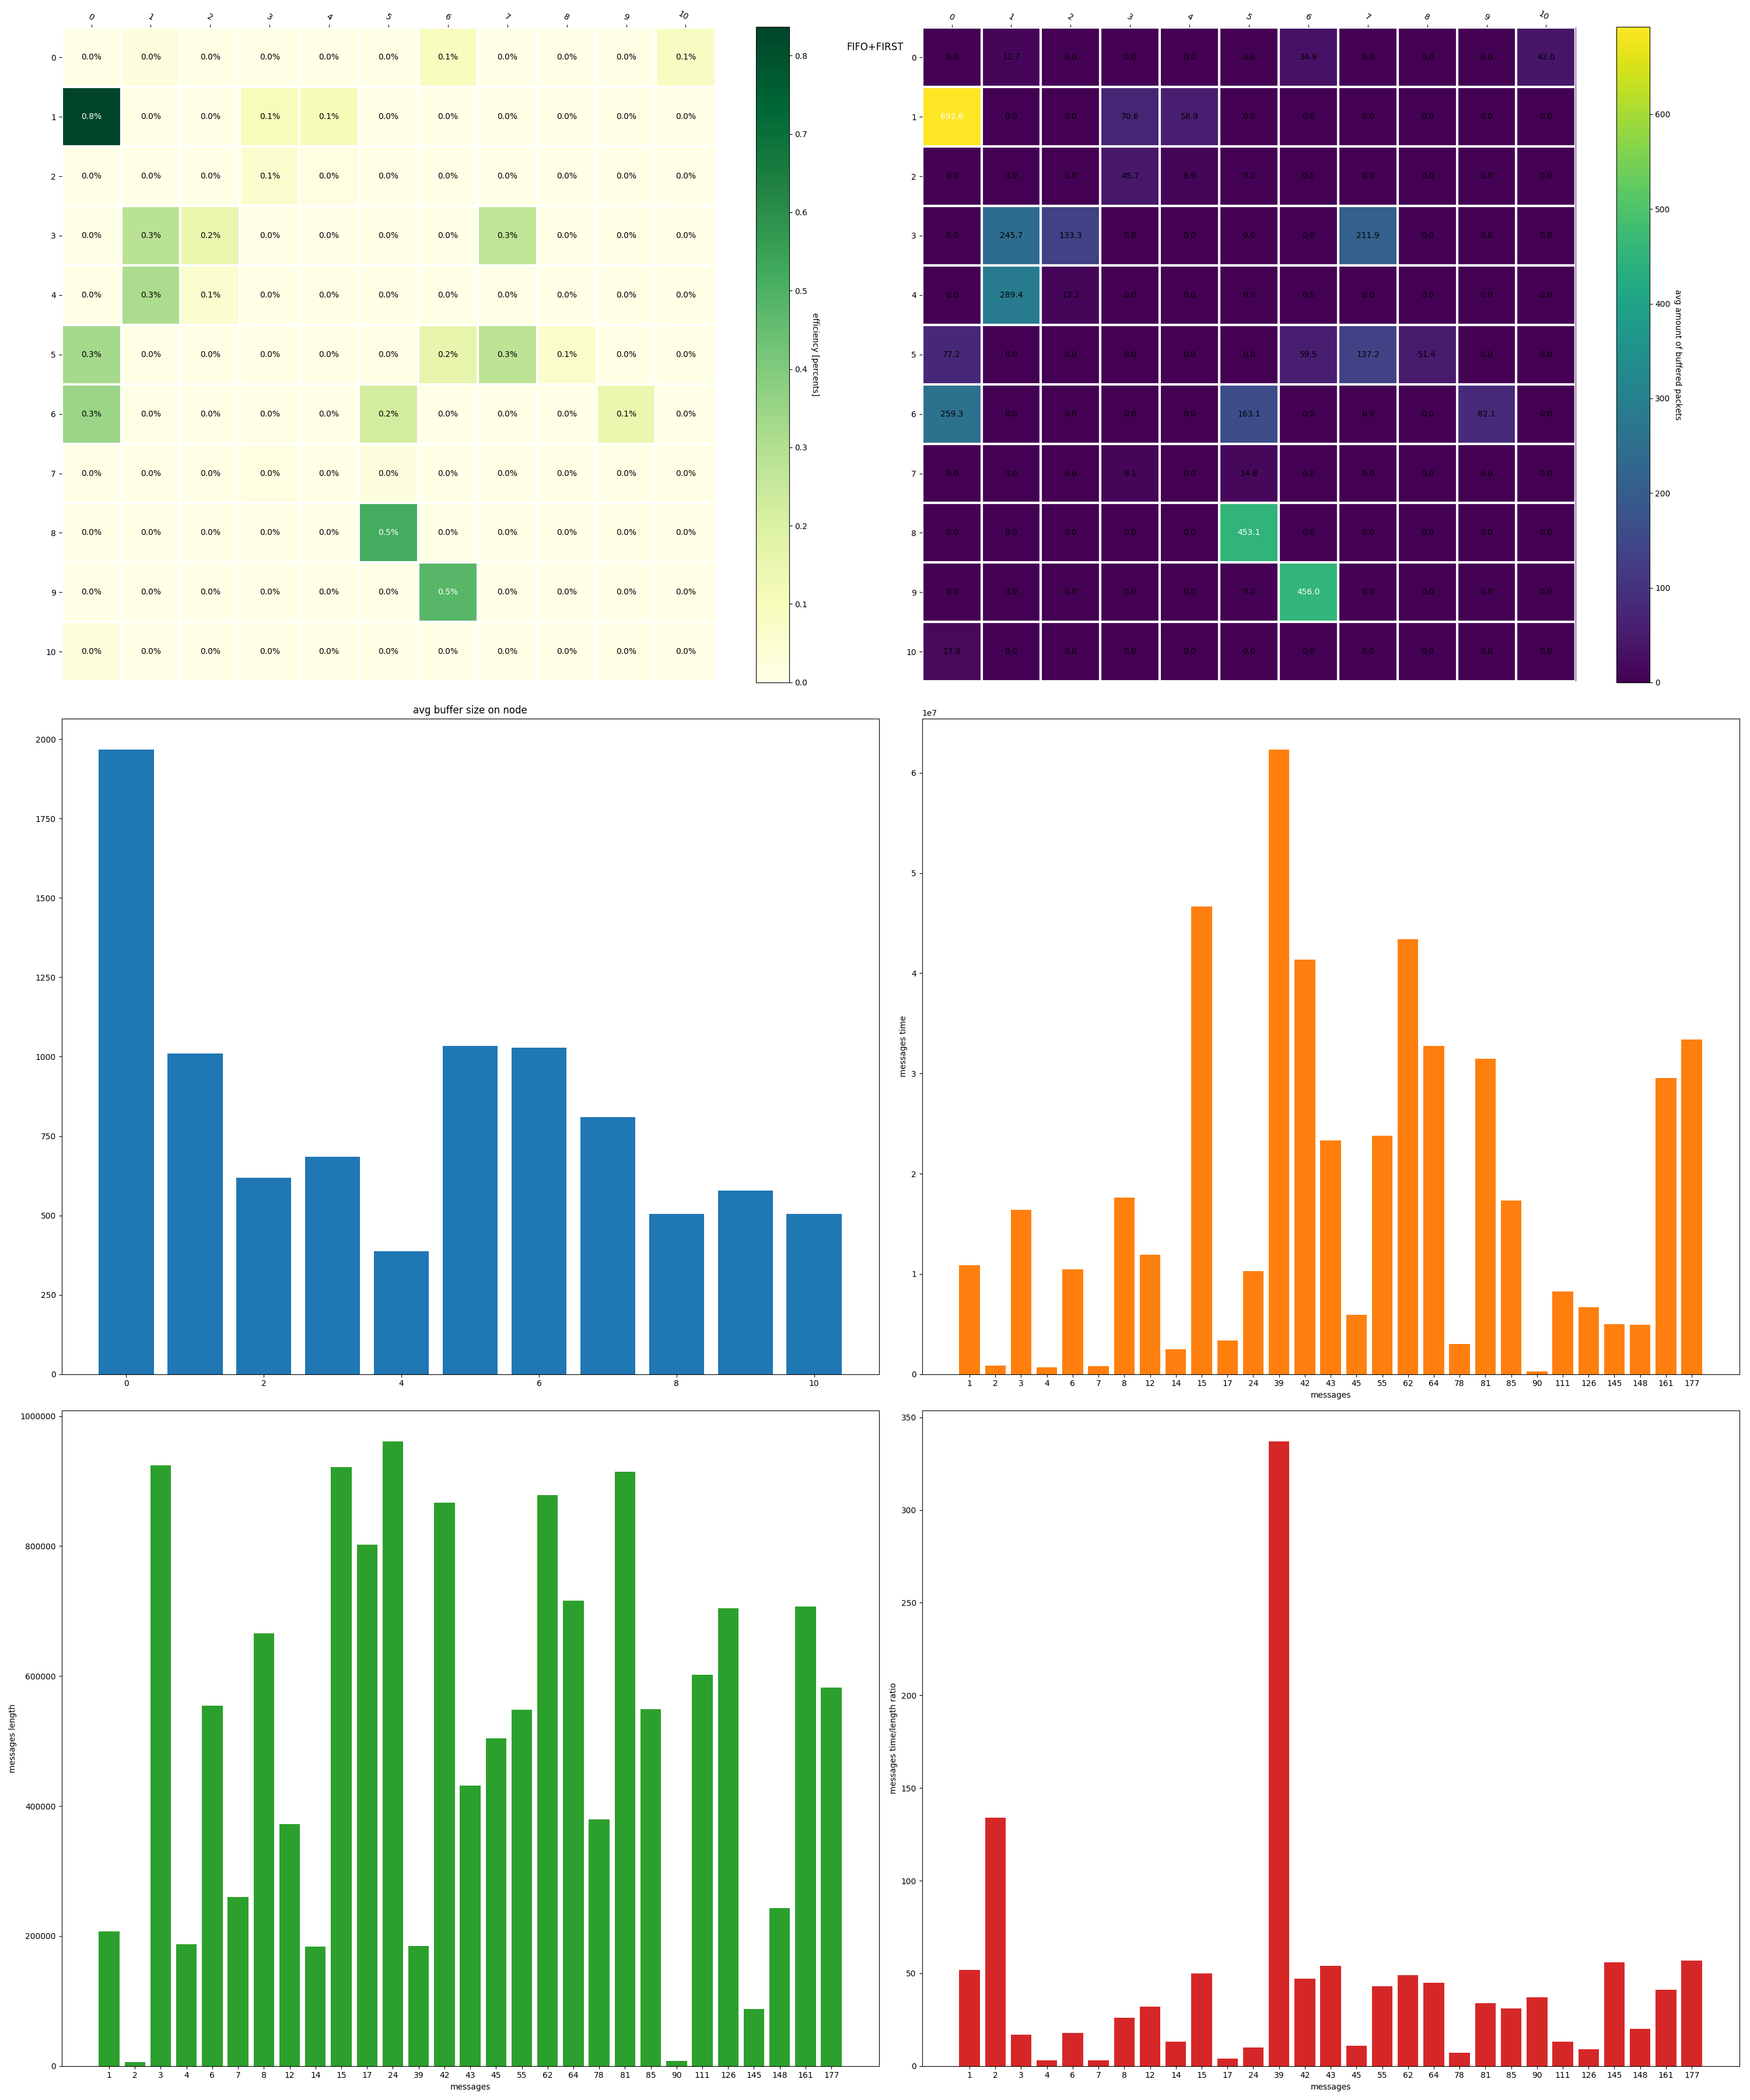
\includegraphics[width=\textwidth]{fifo_first.png}
\caption{FIFO+FIRST}
\end{figure}

\begin{figure}[H]
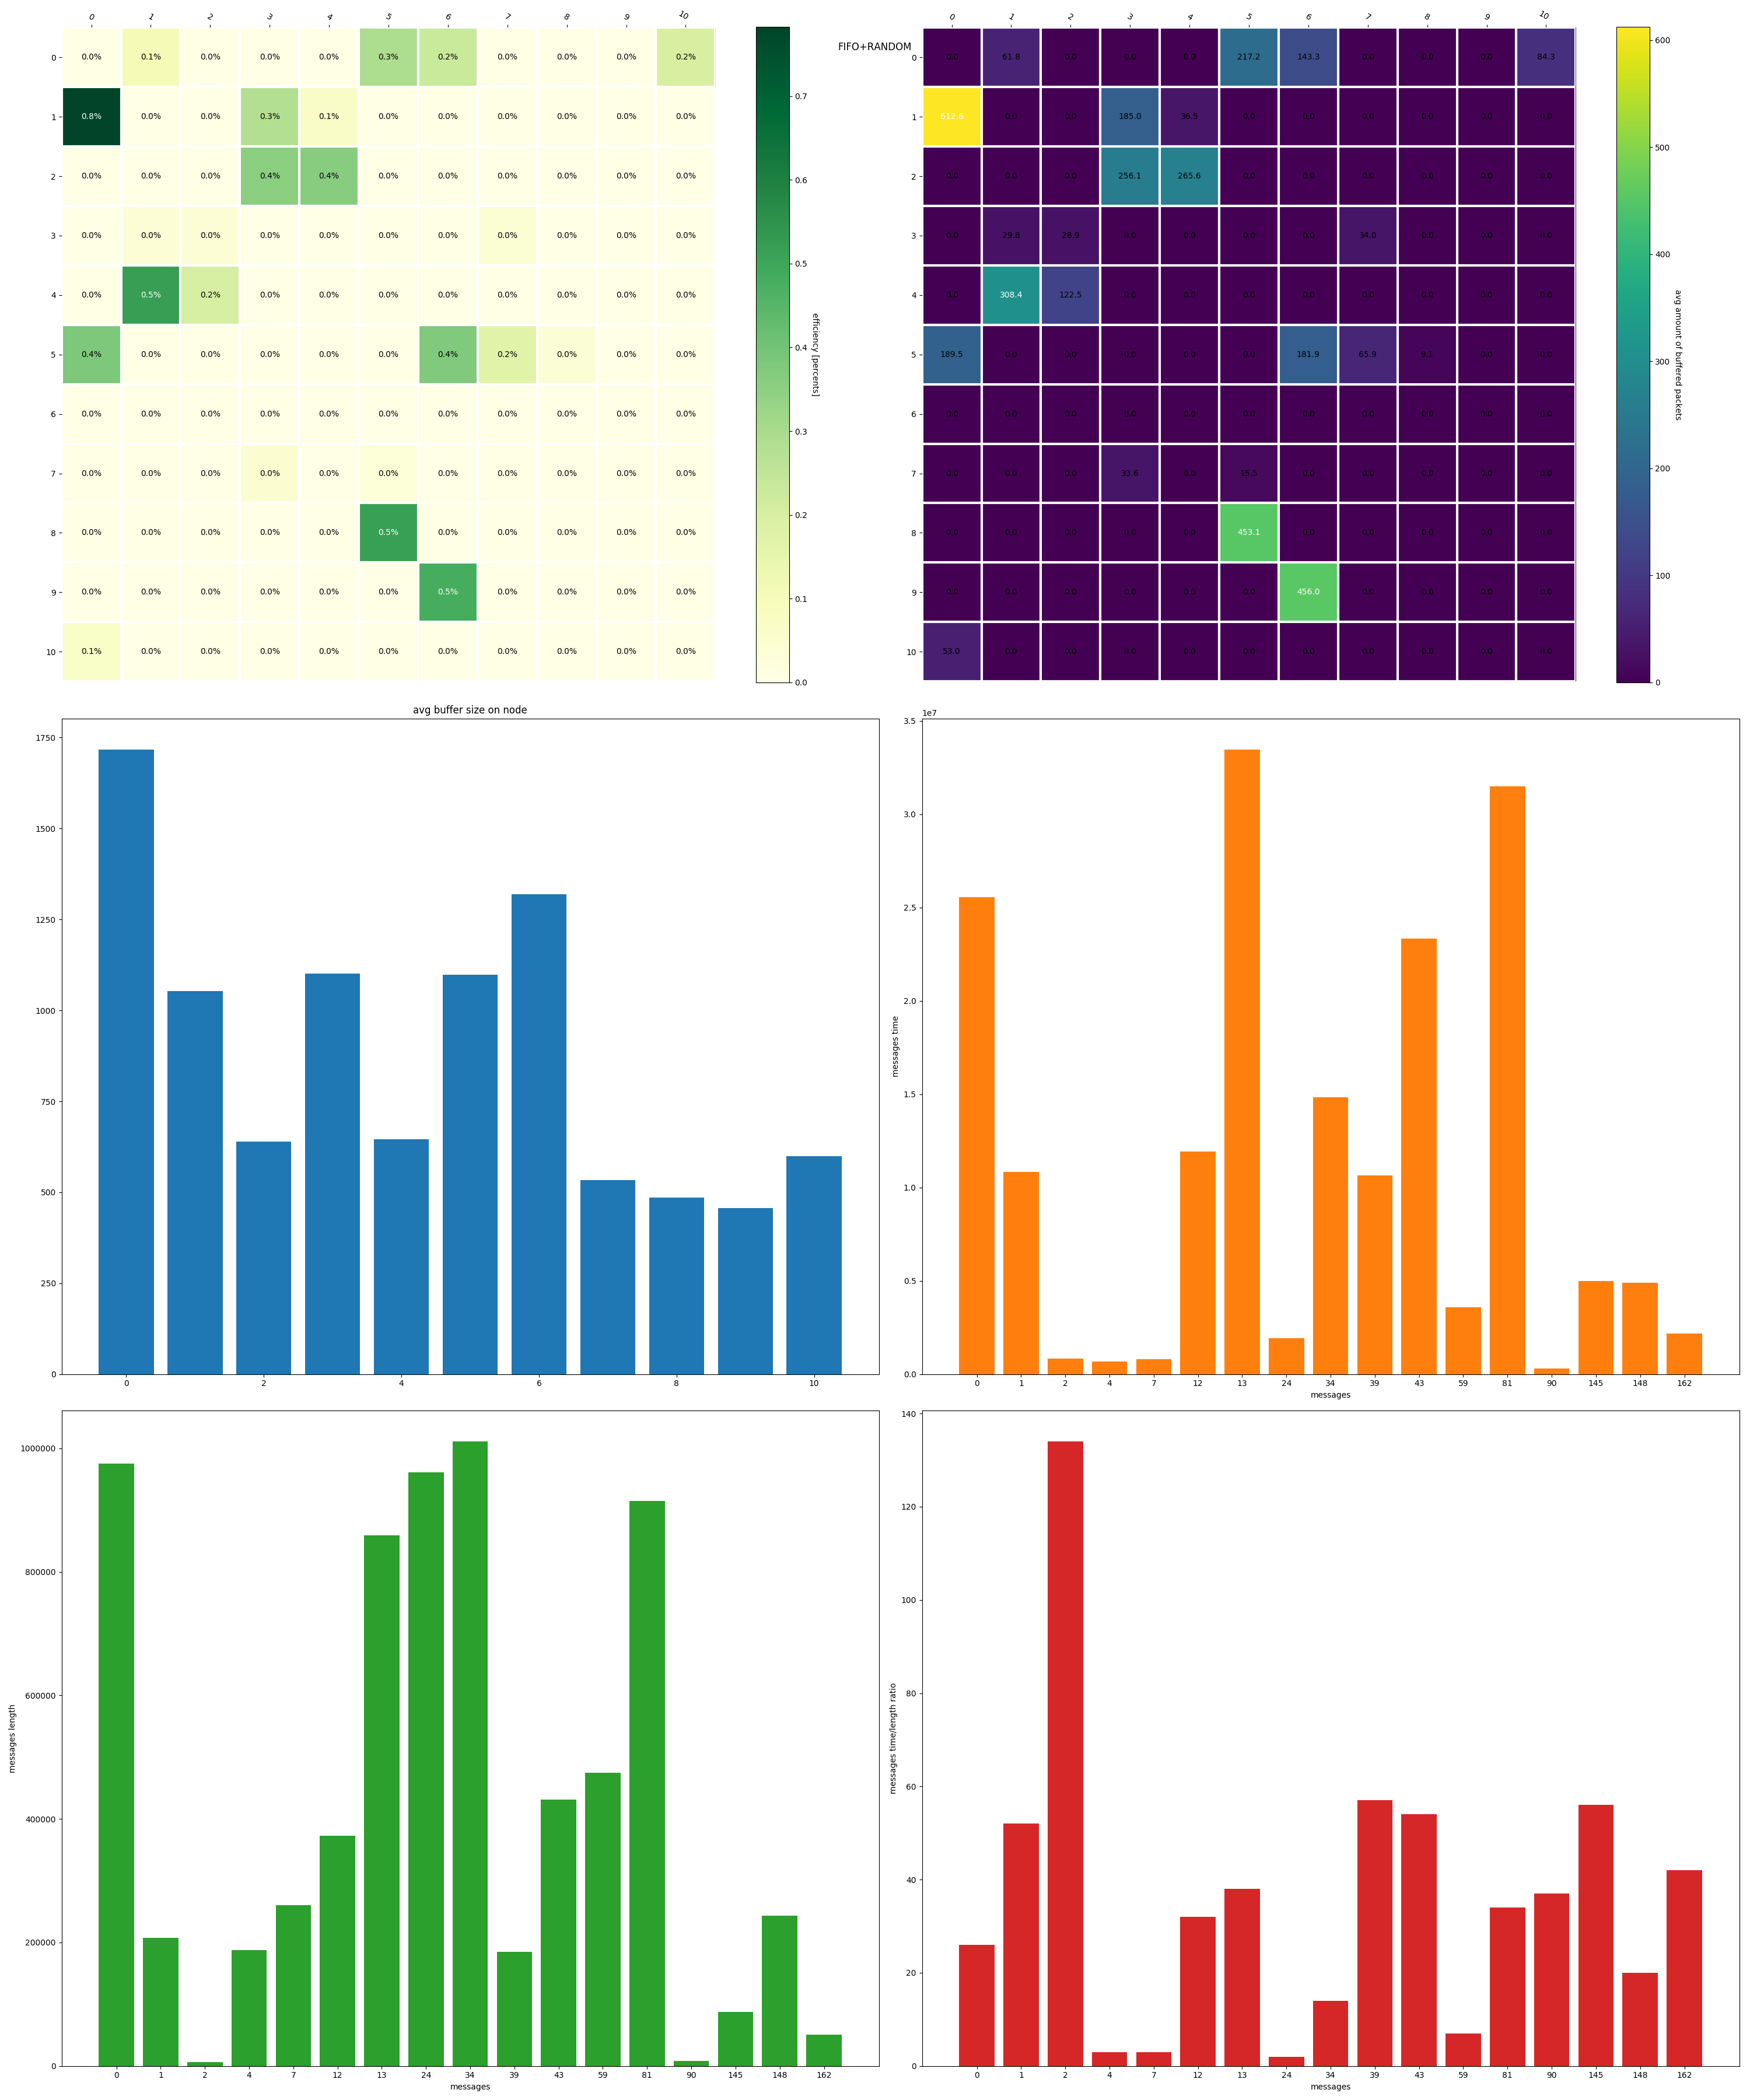
\includegraphics[width=\textwidth]{fifo_random.png}
\caption{FIFO+RANDOM}
\end{figure}

\begin{figure}[H]
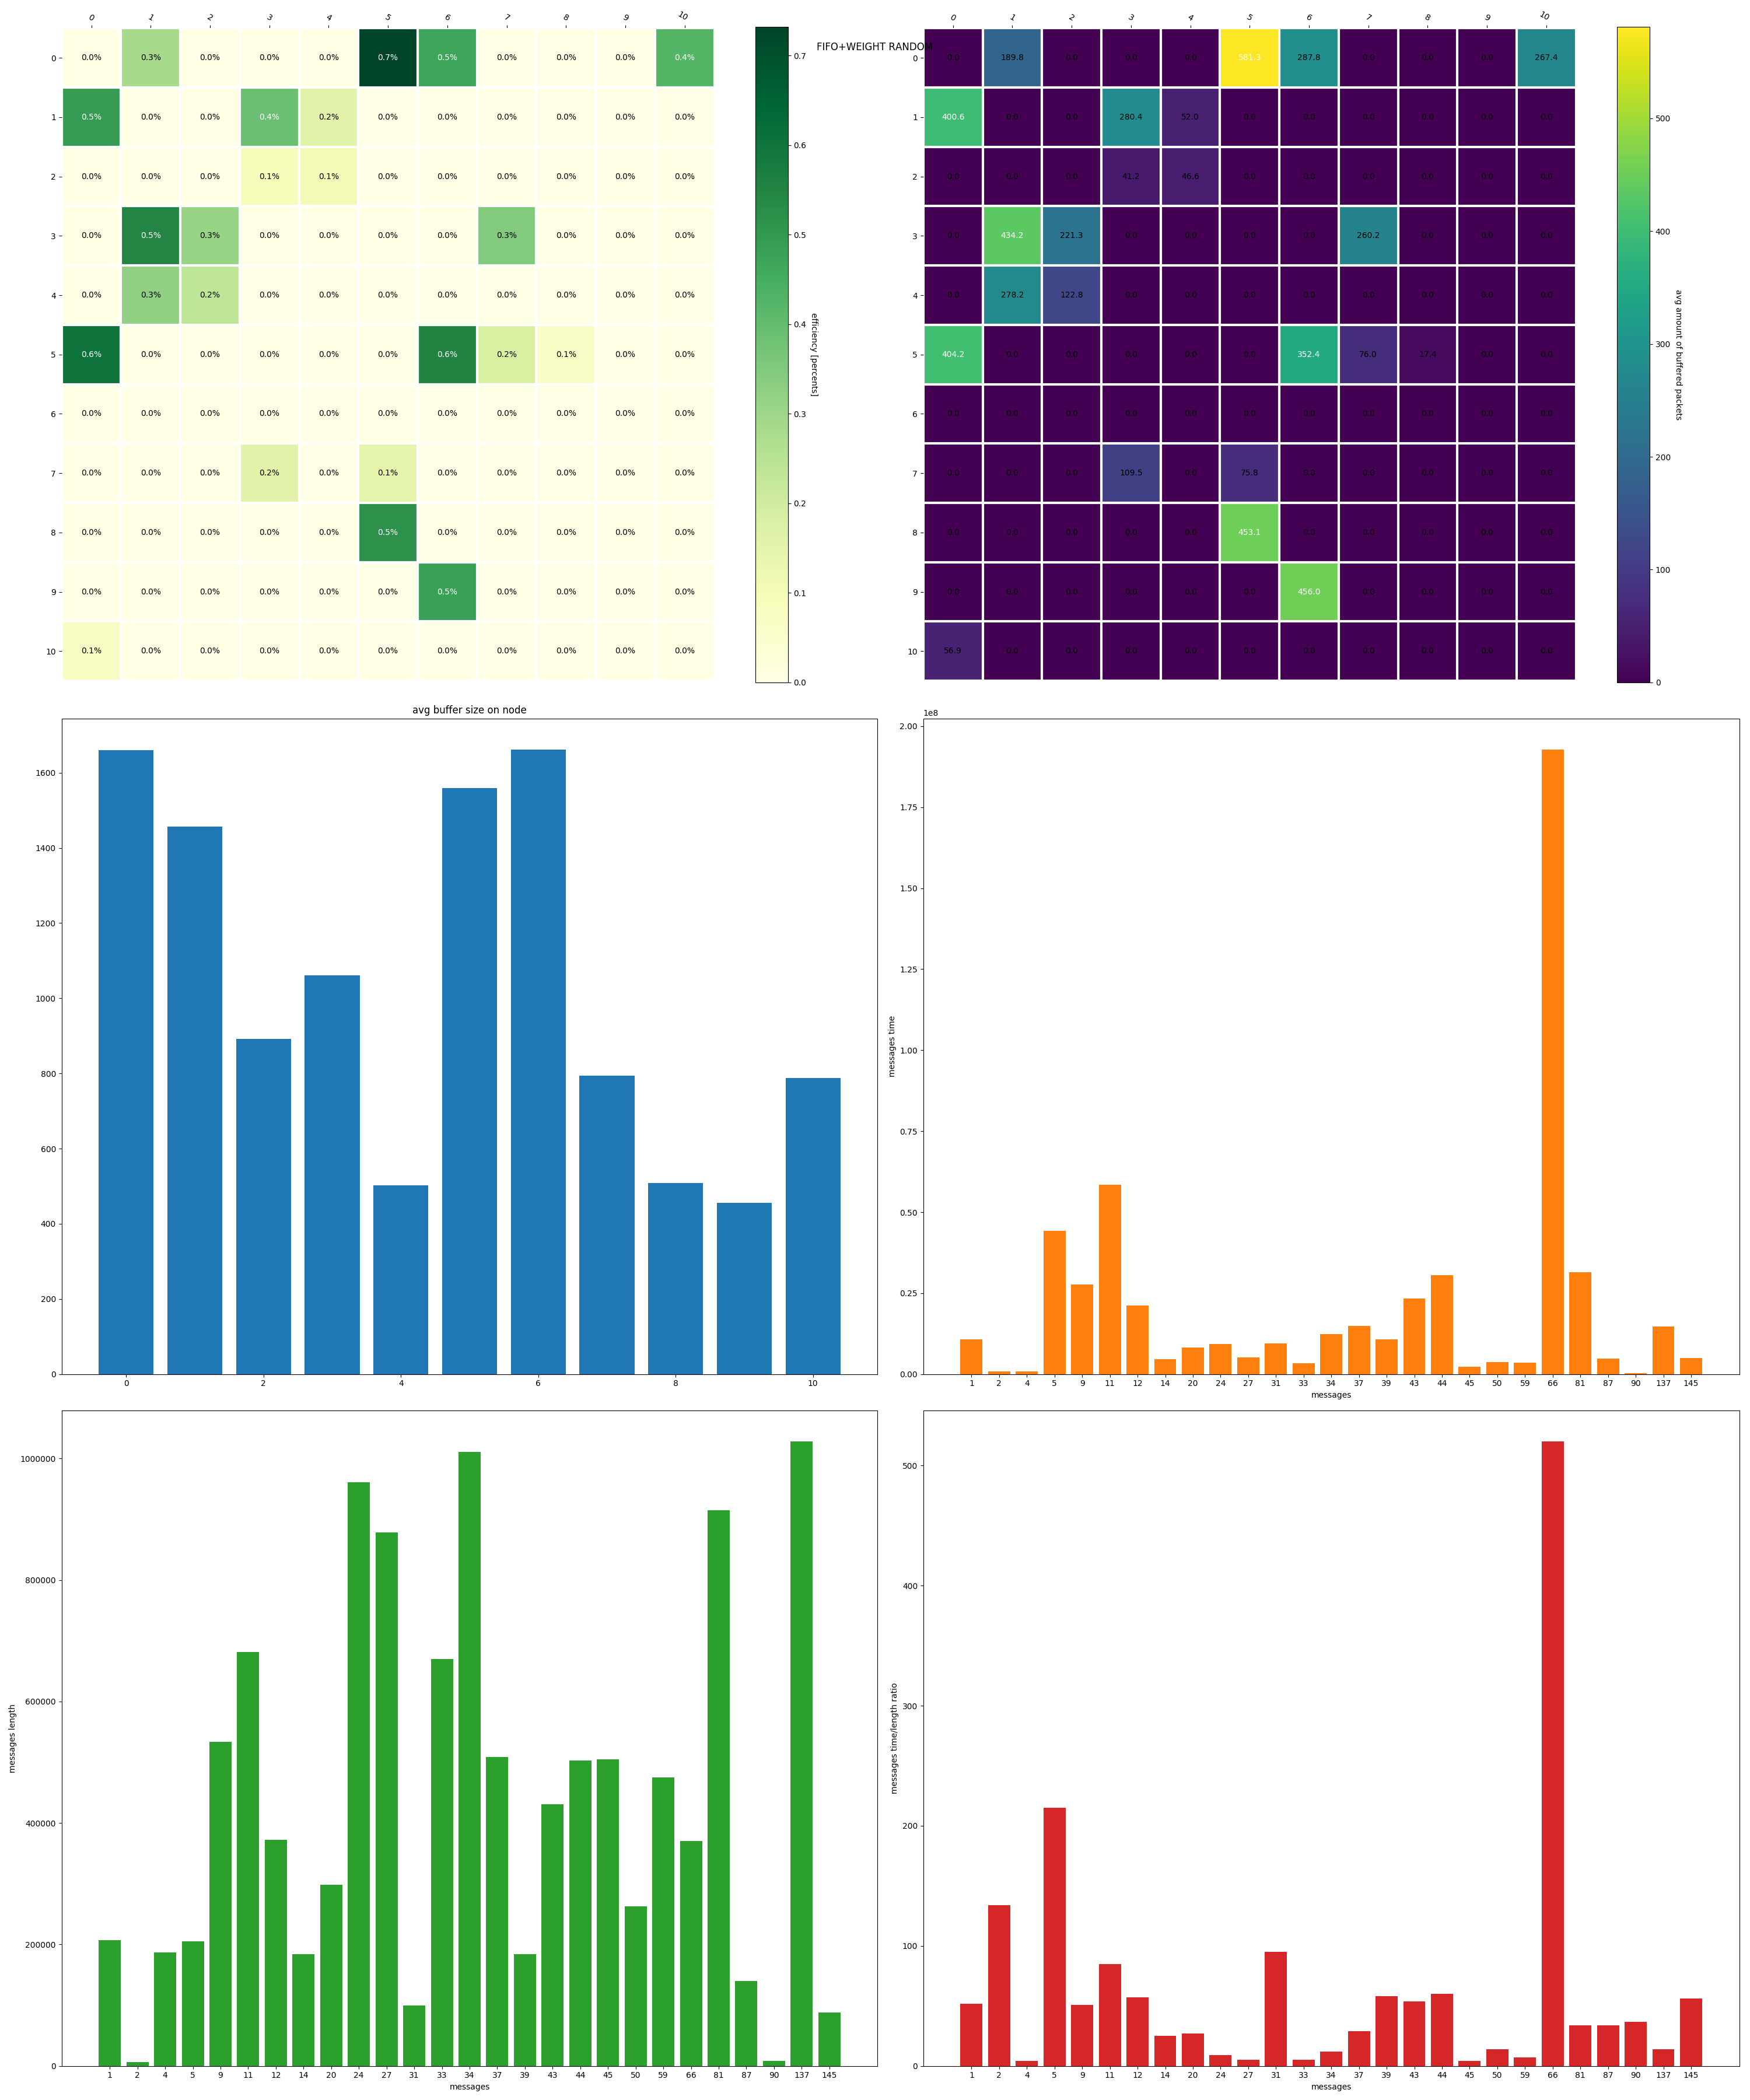
\includegraphics[width=\textwidth]{fifo_weight_random.png}
\caption{FIFO+WEIGHT RANDOM}
\end{figure}

\begin{figure}[H]
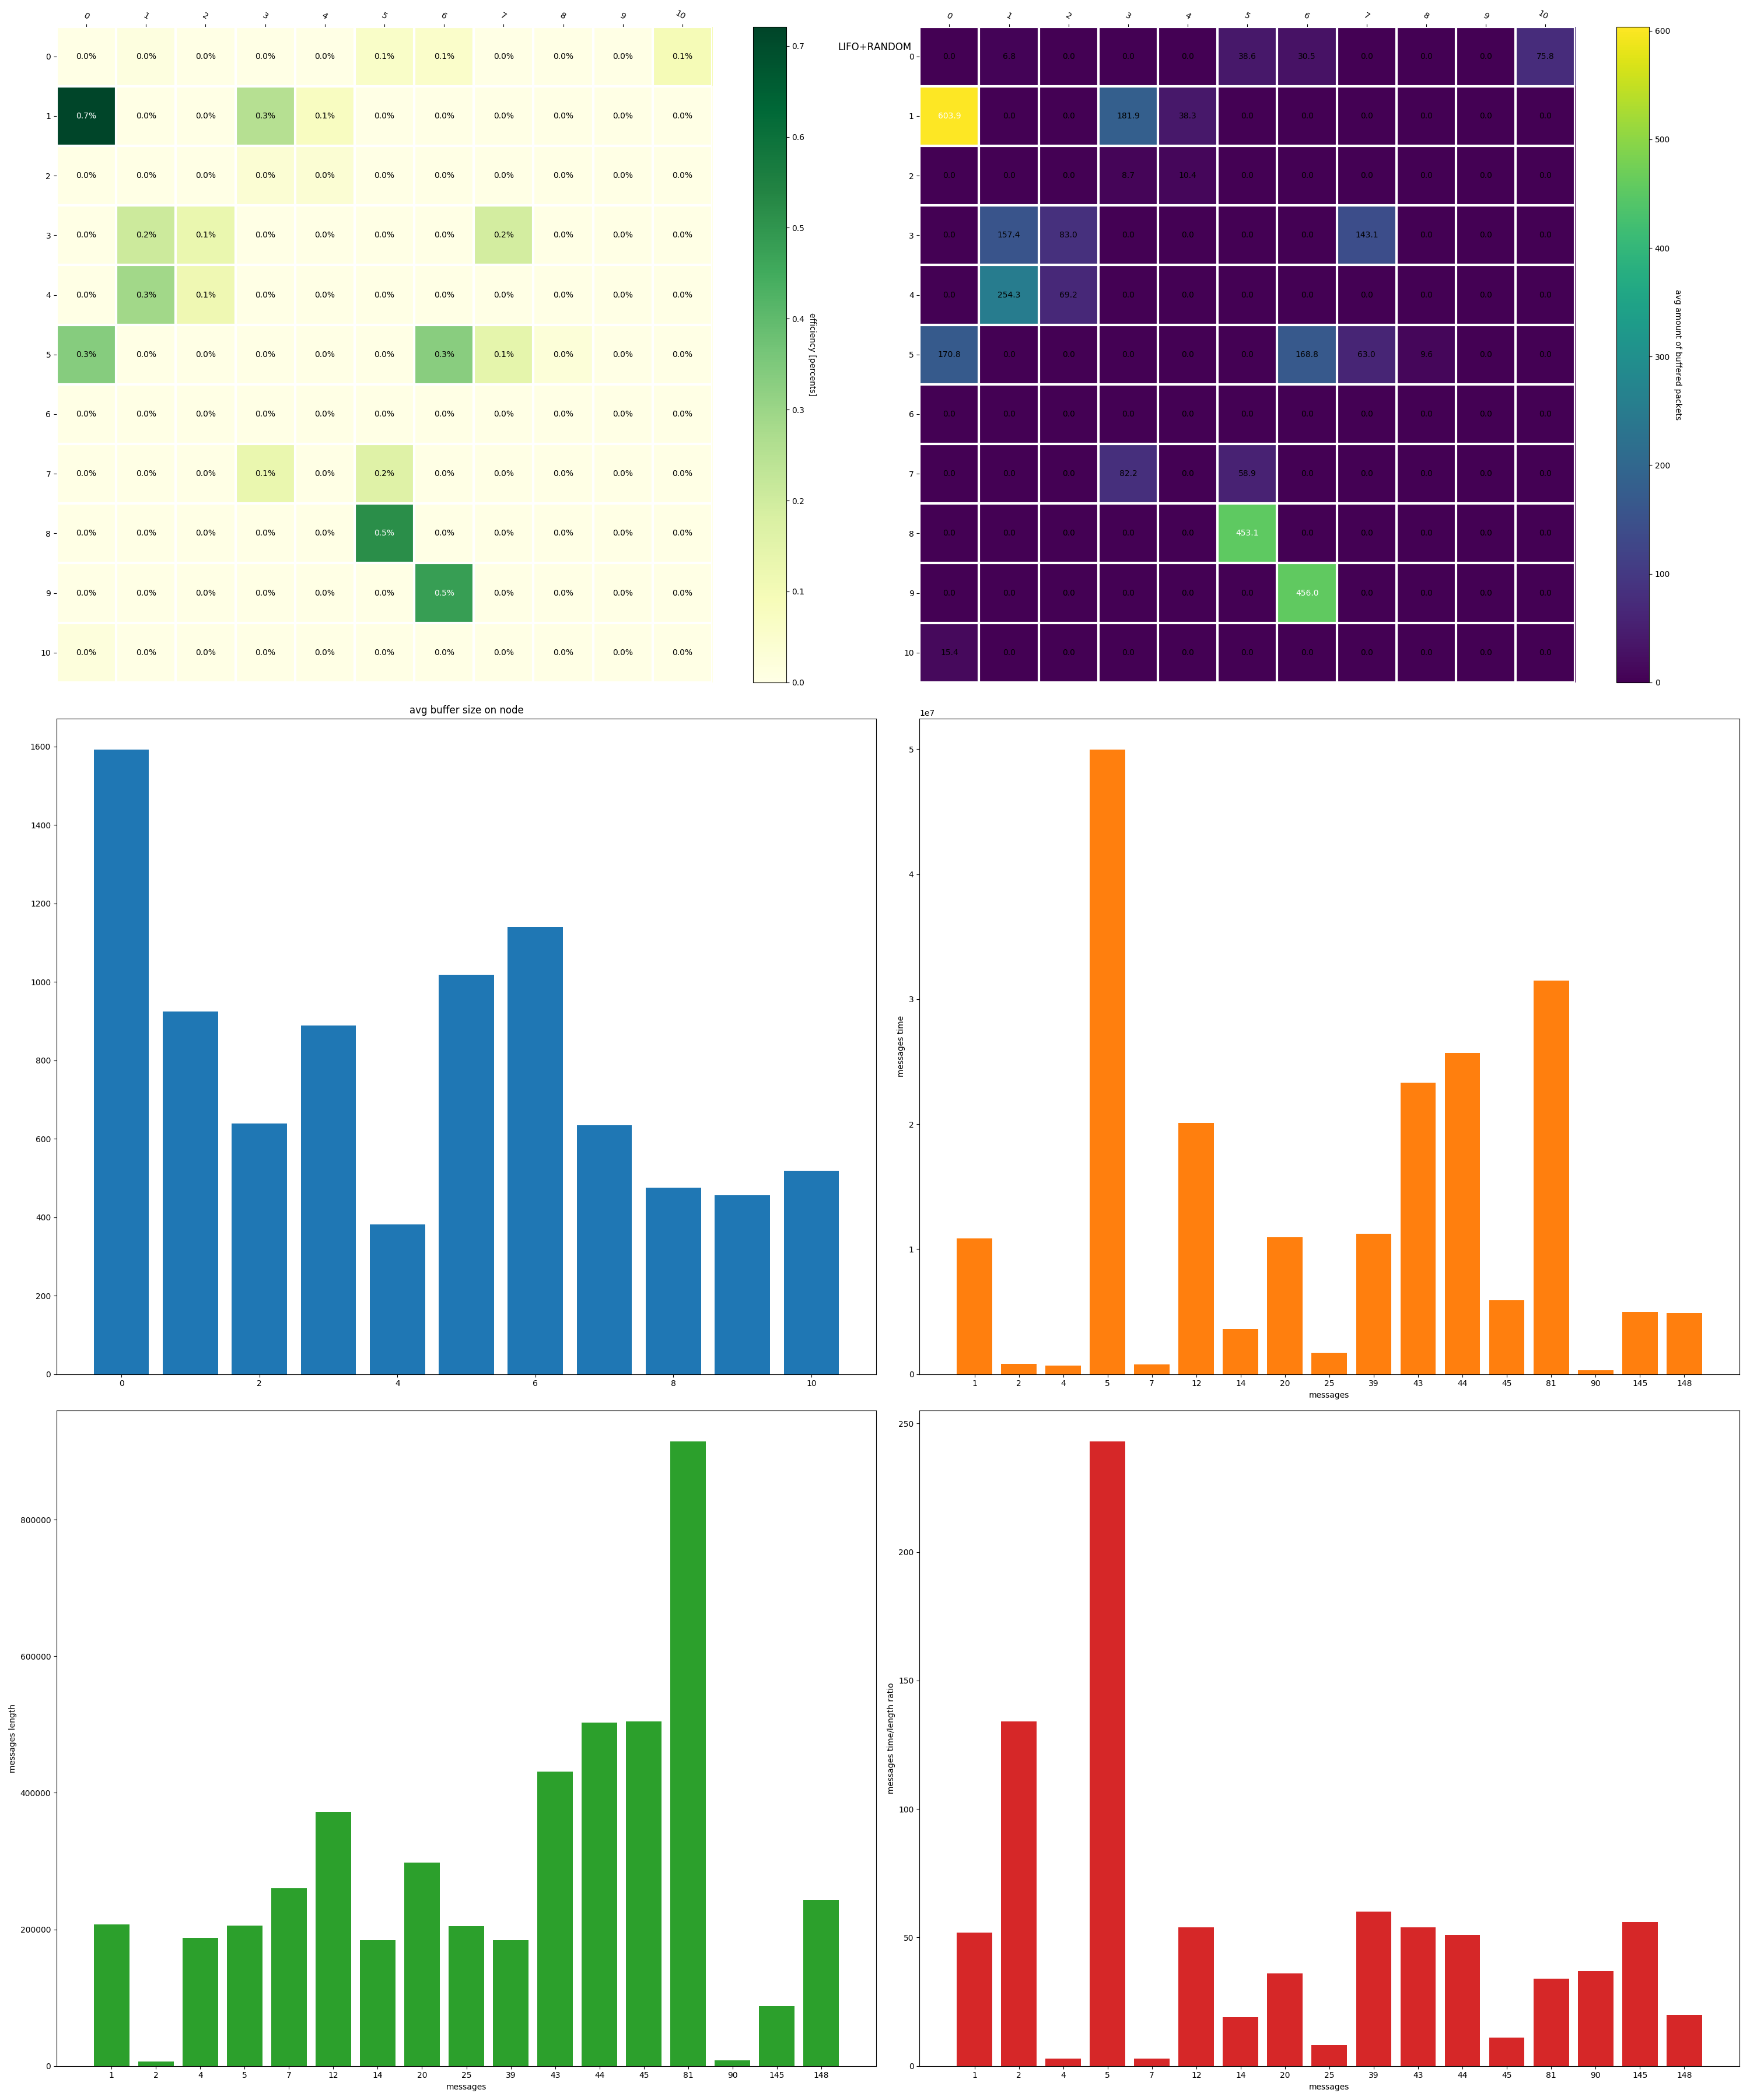
\includegraphics[width=\textwidth]{lifo_random.png}
\caption{LIFO+RANDOM}
\end{figure}

\begin{figure}[H]
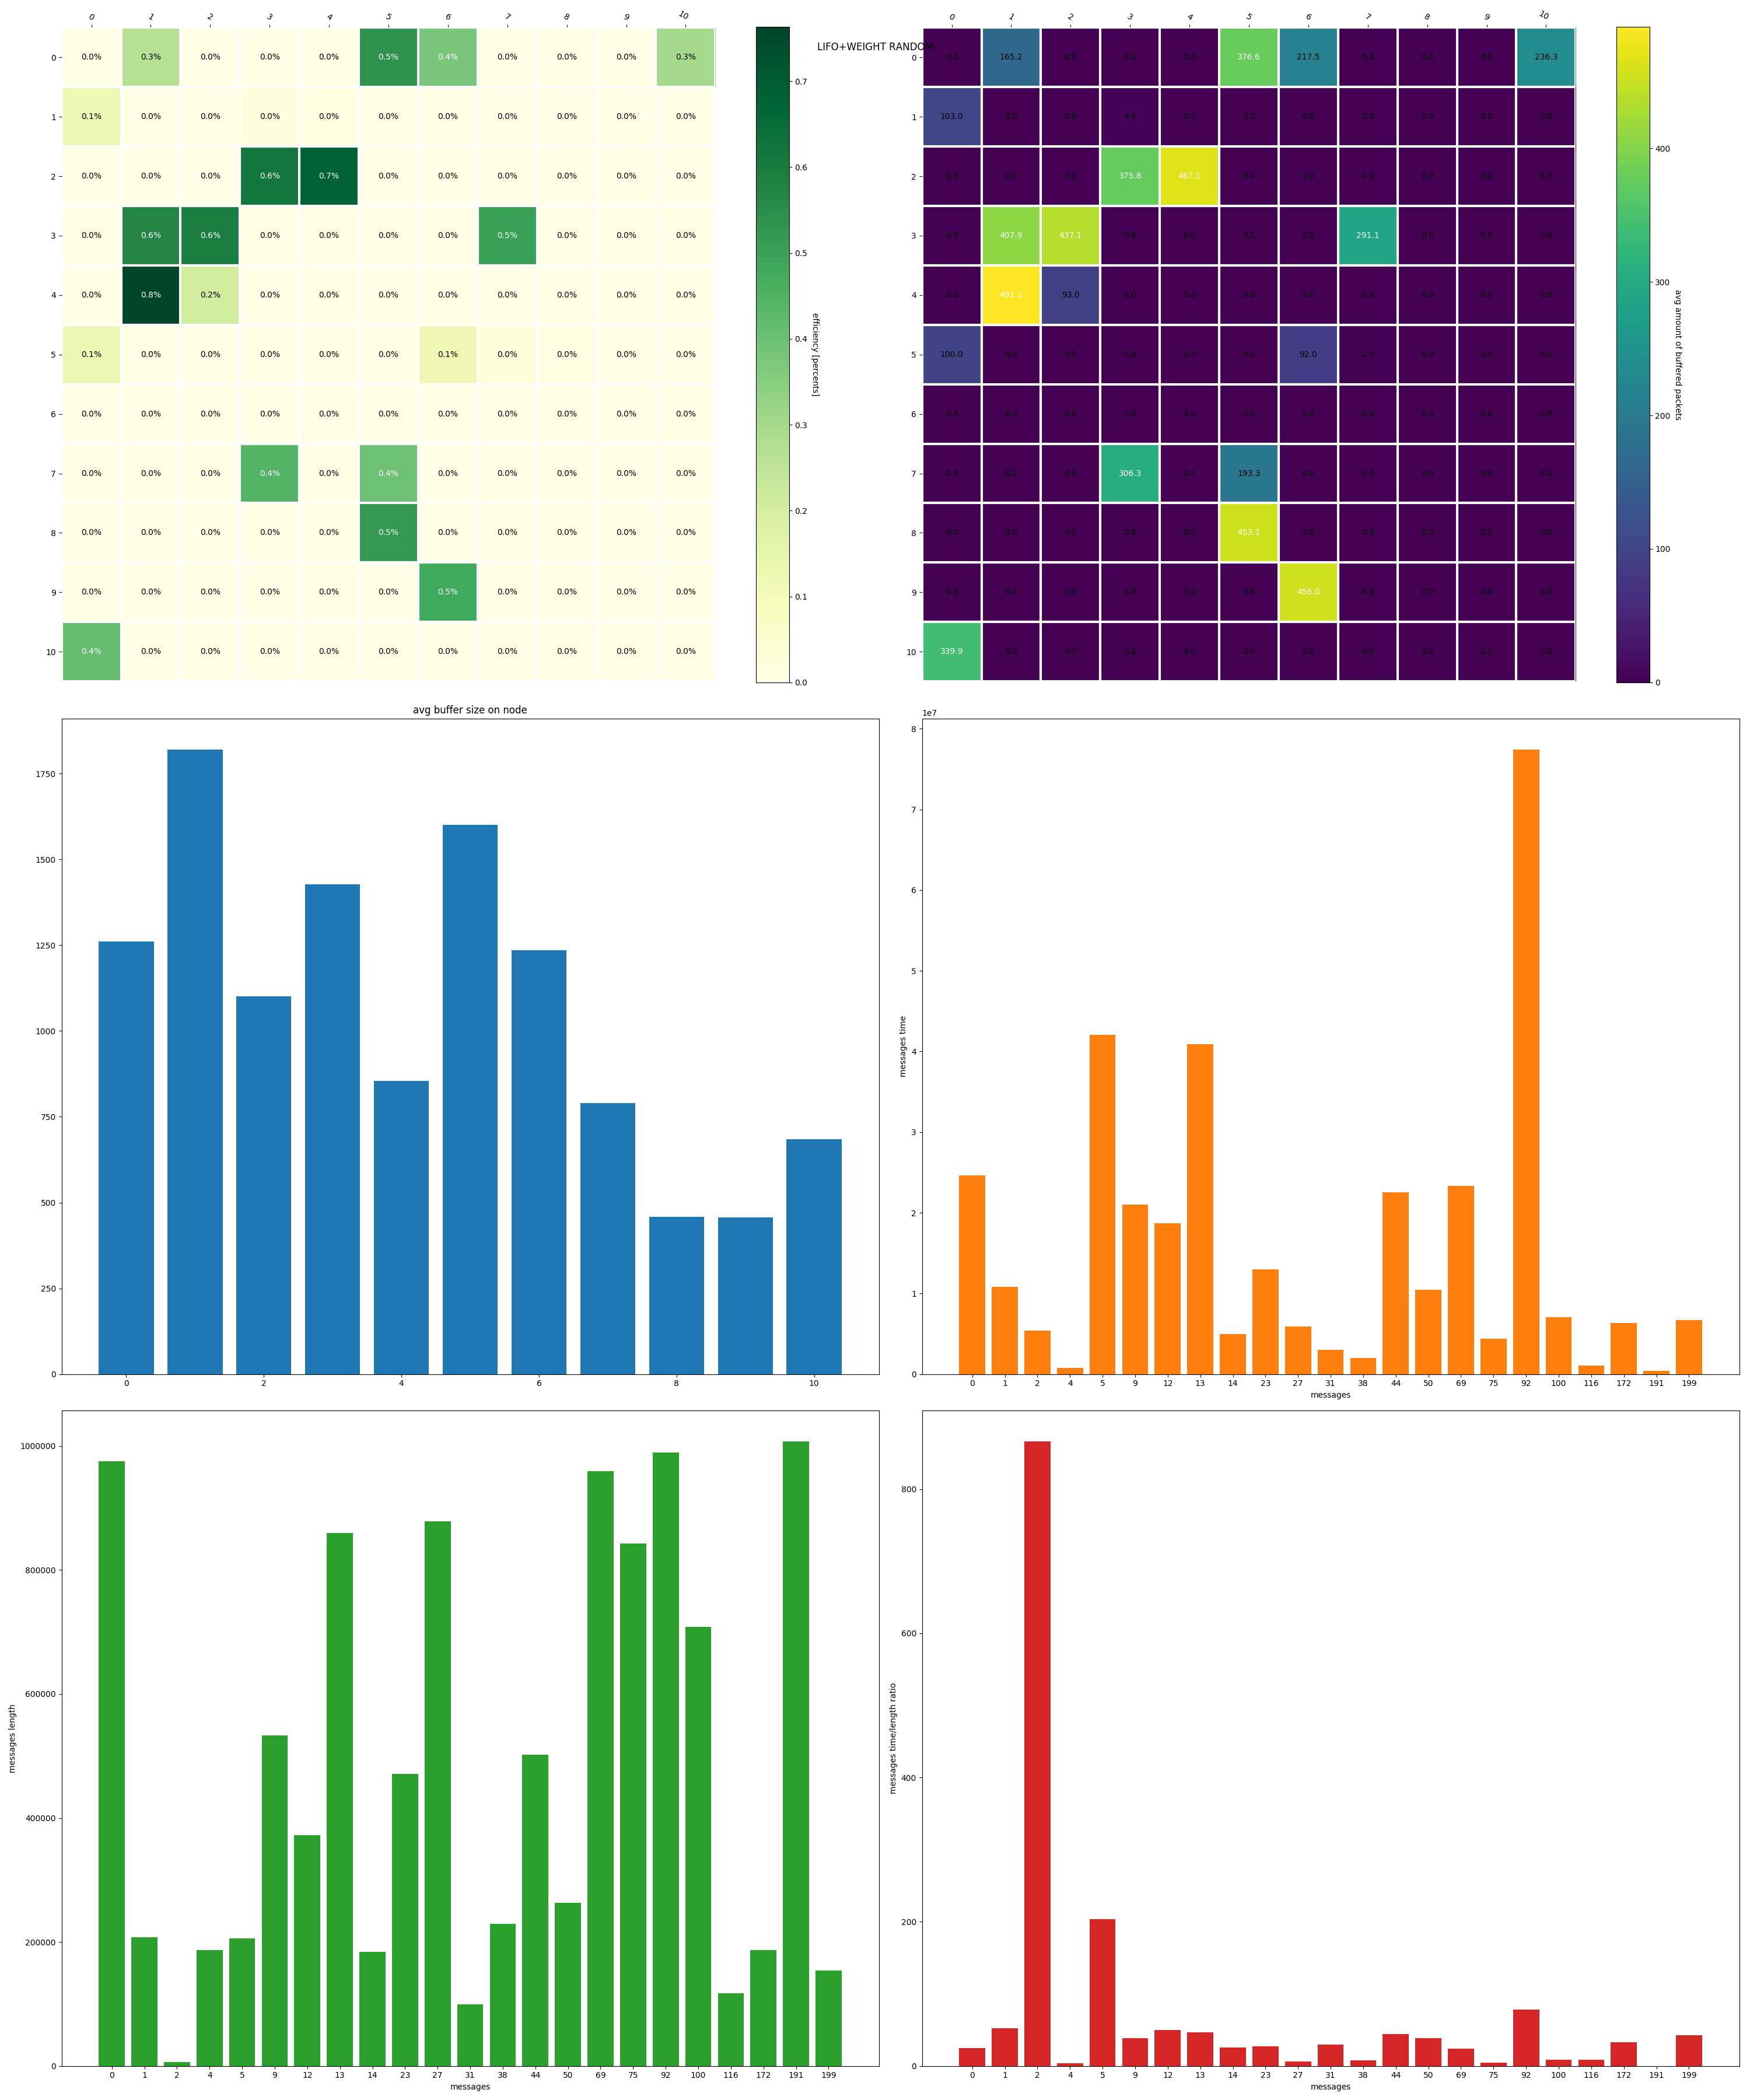
\includegraphics[width=\textwidth]{lifo_weight_random.png}
\caption{LIFO+WEIGHT RANDOM}
\end{figure}

Легенда (зліва напрво, зверху вниз, середні з кроком 50мс):
\begin{itemize}
\item теплова карта ефективності (відношення використання до часу симуляції) каналу;
\item теплова карта середньої кількості буферизованих пакетів у каналах на кожні 50мс;
\item графік середньої кількості буферизованих пакетів на вузлах;
\item графік часу доставлених повідомлень (різниця між часом створення повідомлення і
доставки на вузол);
\item графік довжин доставлених повідомлень (у байтах);
\item графік відношення часу на розмір повідомлення.
\end{itemize}

\begin{figure}[H]
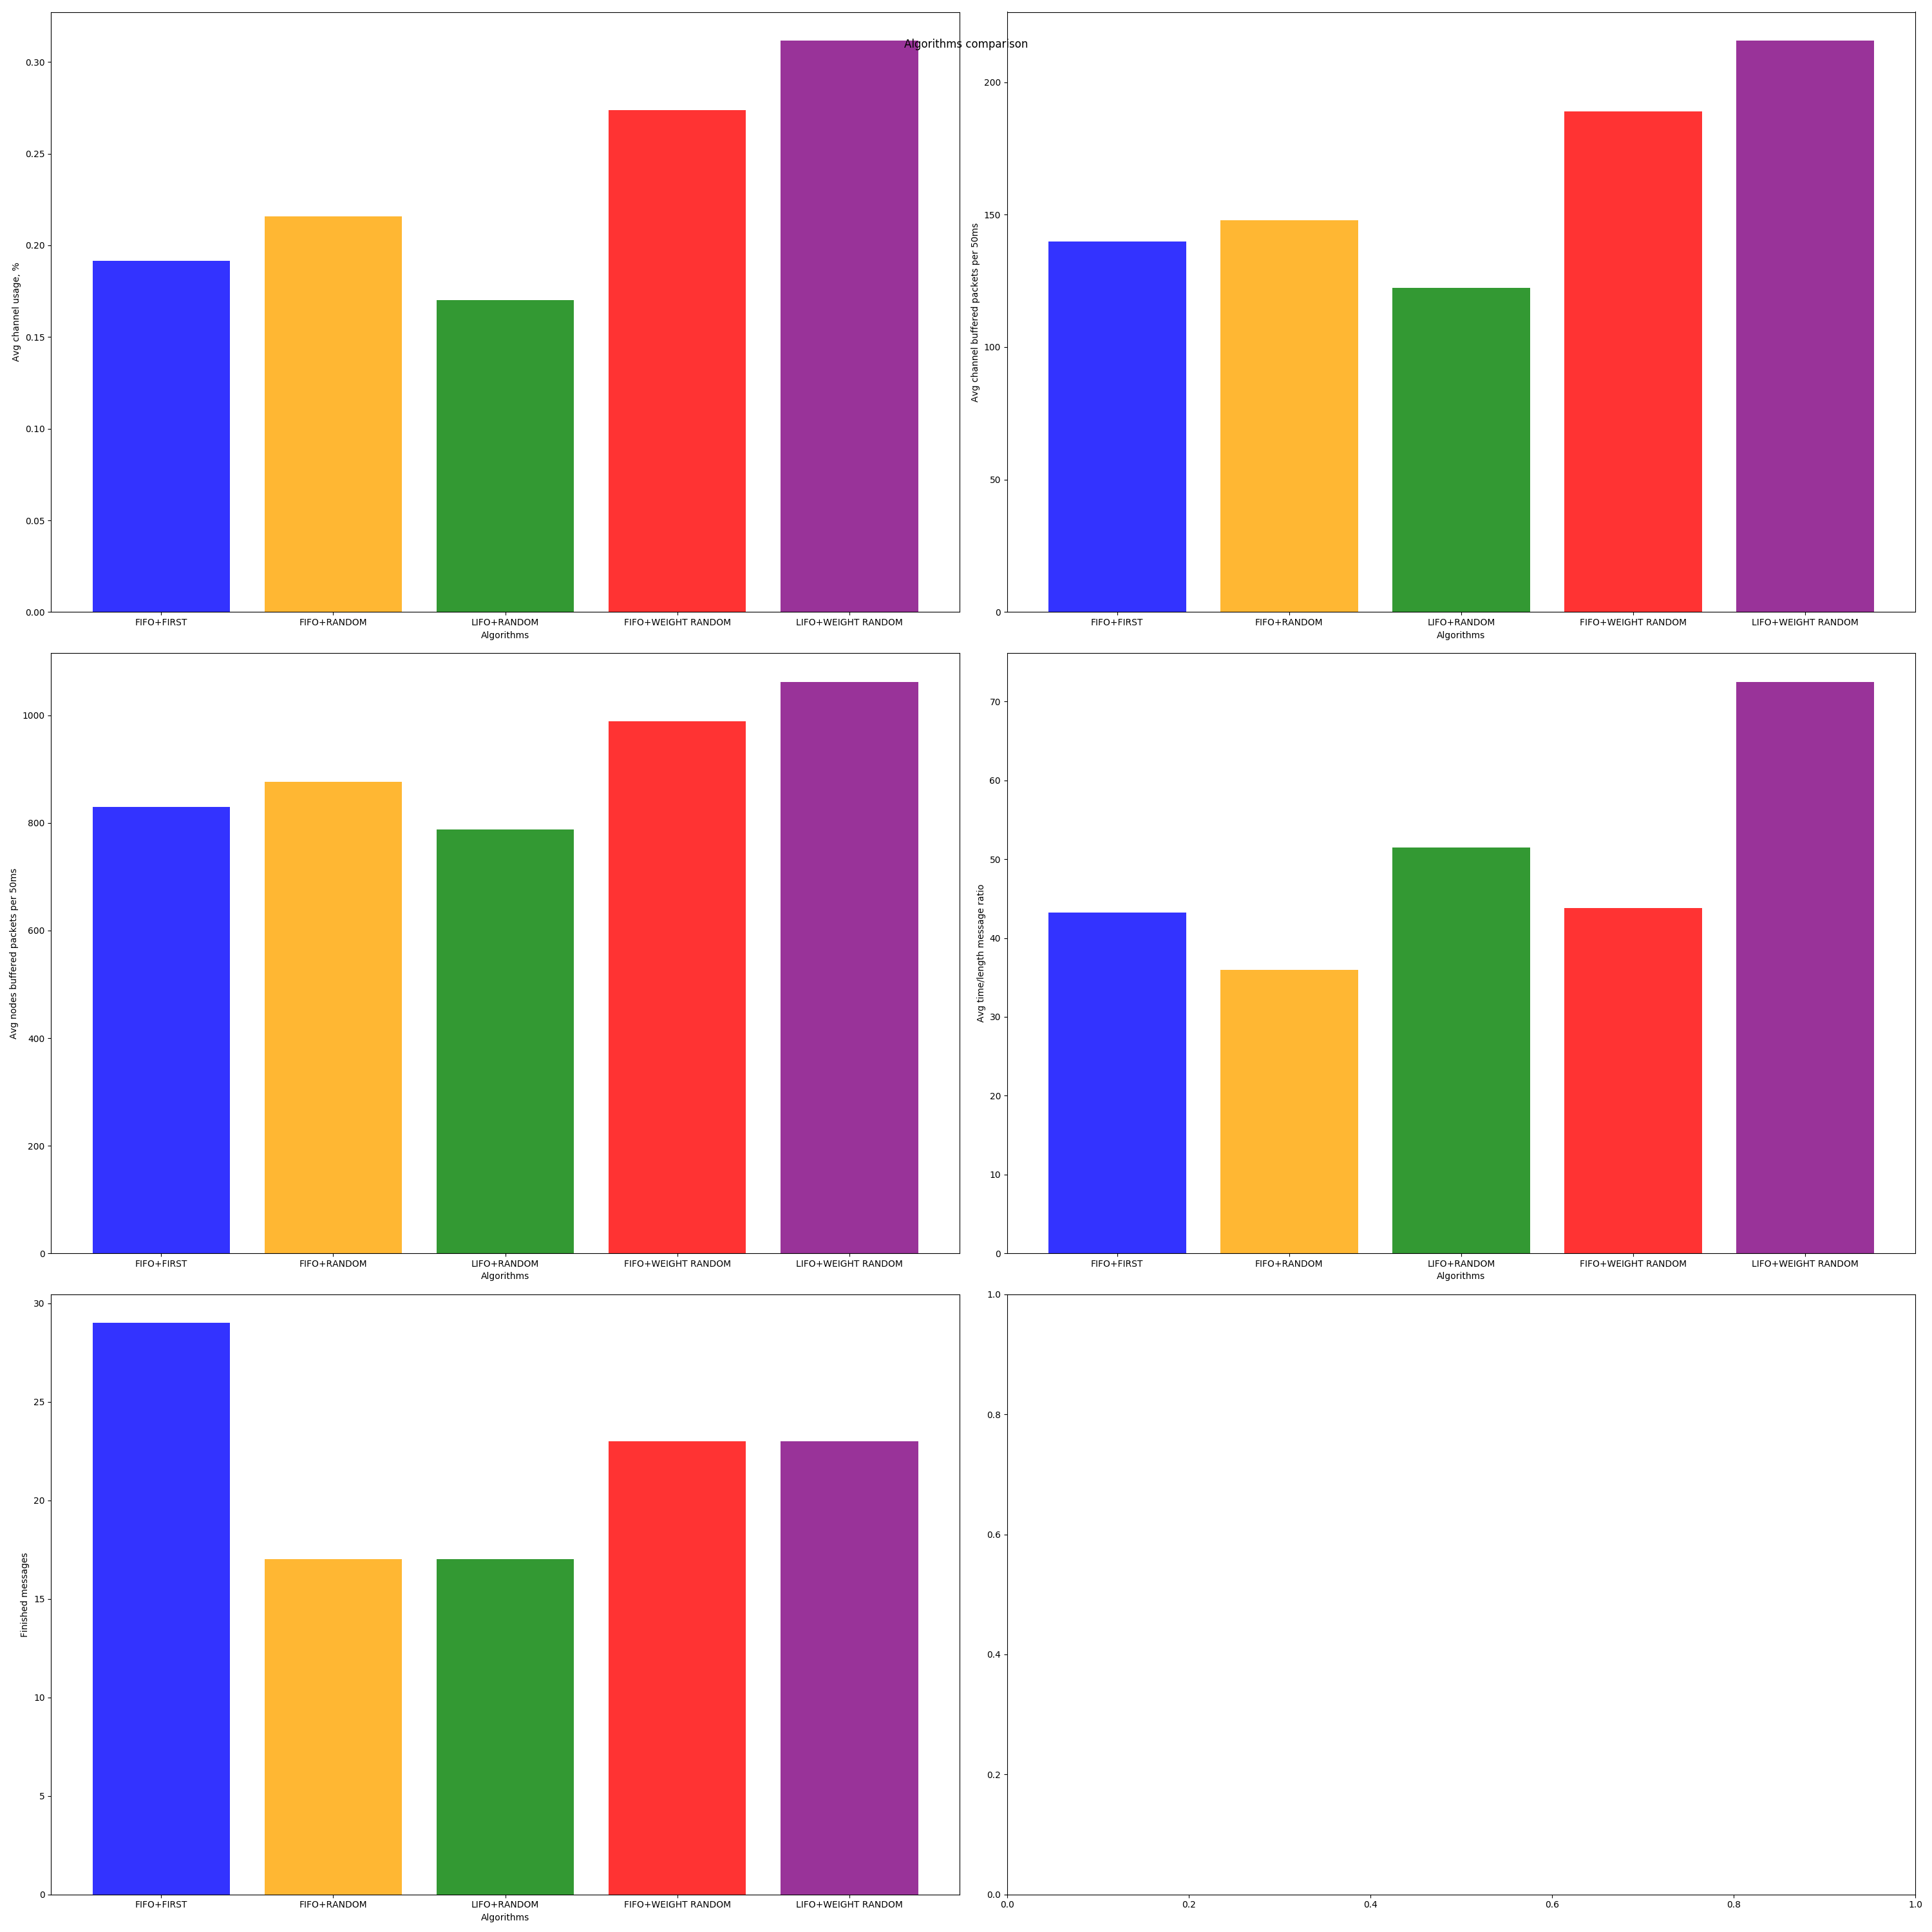
\includegraphics[width=\textwidth]{comparison.png}
\caption{Порівняння}
\end{figure}

Легенда:
\begin{itemize}
\item середня ефективність каналу;
\item середня кількість буферизованих пакетів каналу на кожні 50мс;
\item середня кількість буферизованих пакетів вузла на кожні 50мс;
\item середнє відношення часу до розміру повідомлень (aka latency);
\item кількість доставлених повідомлень за час симуляції.
\end{itemize}

\section{Висновки}

Судячи з наявних результатів, найбільш продуктивною з усіх комбінацій є
\emph{FIFO+WEIGHT RANDOM}. Вона має одну з найбільших значень ефективності каналів 
(вони не простоюють), який добре позначився на загальній кількості 
доставлених повідомлень,гарний latency, але дещо більші значення середньої кількості 
буферизованих пакетів, що
на мою думку спричинено більшим навантаженням на вузли у критичних точках:
вузли 0, 1, 3, 5 та 7 та з'єднуючі їх канали. Такий ефект відбувся тому що вони мають
більший шанс бути задіяними через своє положення у мережі.

Також, непогані результати показує варіант \emph{FIFO+FIRST}, але його ефективність
є скоріш гарним випадком, бо дана мережа дуже проста та одноманітна, тому у цьому конкретному випадку вибір маршруту не настільки критичний.

Більш чіткі та зрозумілі результати можливі лиш за багаторазовою симуляцією
різноманітних, в тому числі незручних для алгоритів, варіантів мереж та трафіку.

У даній же роботі був розглянутий лиш найпростіший варіант трафіку і мережі.

\section{Можливі поліпшення}

Даній симуляції бракує динамічної зміни таблиць маршрутизації (яка є ключовим моментом оптимізації
навантаження, але є найбільшою складністю для симуляції насамперед з точки зору складності реалізації)
та більш тонкого налаштування мережі: дана мережа достатньо статична, тоді
як у реальних різні вузли мають різні характеристики (швидкість обробки, ліміти пам'яті), 
канали мають разні швидкості,
як для різних пар вузлів, так і для зворотніх з'єднаннь між двома вузлами (більша швидкість
на завантаження, ніж на вивантаження, наприклад).
Дані можливості вже доступні всередині рушія, але не можуть бути налаштовані ззовні
так як потребують ґрунтовної роботи з перевірки коректності усіх цих параметрів
та відшліфування їх інтерфейсів, що, нажаль, не зроблено через брак часу.

У мережі також відсутній такий вид трафіку, як \emph{TCP} (наразі симулюється по суті лиш
\emph{UDP}), який є важливим елементом сучасних мереж, і його симуляція є корисною. Також
це дозволило би симуляцію змішаного навантаження, \emph{TCP} разом з \emph{UDP}.

Також можна було би симулювати різні типи навантаження, а точніше різних типів застосунків, базуючись на деяких рисах вузлів, наприклад, сервери популярного сервісу, на який симулюється сильне навантаження, а також супутній трафік, непов'язаним з сервісом.
\end{document}
